\subsection{Вітчизняний досвід використання імерсивних освітніх ресурсів у професійній підготовці майбутніх учителів інформатики}\label{subsec:1.3}

З метою вивчення та узагальнення наявного вітчизняного досвіду використання імерсивних освітніх ресурсів у підготовці майбутніх учителів інформатики було здійснено аналіз офіційних сайтів провідних закладів вищої освіти України, у яких реалізуються освітні програми з підготовки фахівців відповідного профілю. Увагу зосереджено на змісті освітньо-професійних програм, навчальних планах, описах освітніх компонентів, матеріалах навчально-методичного забезпечення, а також на відкритих інформаційних ресурсах, що відображають практики використання цифрових та імерсивних технологій у професійній підготовці майбутніх учителів інформатики.

\textbf{Міжнародний контекст інтеграції імерсивних технологій у педагогічну освіту.} Перш ніж звернутися до вітчизняного досвіду, доцільно окреслити загальносвітові тенденції впровадження XR-технологій у підготовку вчителів, що слугуватиме порівняльною рамкою для подальшого аналізу.

Систематичний огляд 52 досліджень, проведений Y.~Wang та X.~Li~\cite{Angelov2025Synergy}, засвідчив, що у світовій практиці XR-технології в педагогічній освіті використовуються переважно для формування процедурних знань і навичок, причому VR залишається найпоширенішим інструментом, а цільовою аудиторією є здебільшого студенти педагогічних спеціальностей (pre-service teachers). SWOT-аналіз виявив ключову слабкість: відсутність теоретично обґрунтованого дидактичного дизайну XR-ресурсів. Суттєво, що в більшості досліджень майбутні вчителі виступають \emph{користувачами} імерсивних технологій, а не їх \emph{розробниками}, --- ця глобальна тенденція безпосередньо корелює з виявленим нижче українським розривом між технологічним потенціалом і педагогічною реалізацією.

Дослідження S.~Taggart et~al.~\cite{Taggart2023Makers} показало, що навіть короткочасні інтервенції з використанням VR/AR підвищують самоефективність і позитивне ставлення майбутніх учителів до імерсивних технологій (Ірландія, Велика Британія), однак основними бар'єрами залишаються швидкість технологічних змін, відсутність часу для глибокого освоєння та обмежене фінансування~--- фактори, що суттєво резонують з українськими реаліями. У контексті країн, що розвиваються, M.~Nikimaleki та M.~Rahimi~\cite{Nikimaleki2022CollaborativeAR} продемонстрували, що колаборативне AR-навчання на основі конструктивістської педагогіки значно підвищує навчальні результати та впевненість у застосуванні технологій навіть за обмежених ресурсних умов. Водночас K.~Bucher та S.~Grafe~\cite{Bucher2018DesigningARVR} одними з перших апробували підхід, за якого студенти педагогічних спеціальностей самостійно проєктували AR/VR-додатки, що засвідчило принципову можливість переходу від моделі <<вчитель як користувач>> до моделі <<вчитель як розробник>> імерсивних ресурсів.

Отже, міжнародний досвід засвідчує: (1)~проблема підготовки вчителів як розробників ІОР є глобальною, а не суто українською; (2)~навіть обмежені за часом і ресурсами інтервенції дають позитивні результати; (3)~відсутність теоретично обґрунтованої методики залишається центральним бар'єром у всіх досліджуваних контекстах. Ці висновки визначають аналітичну перспективу для подальшого розгляду вітчизняного досвіду.

\textbf{Нормативно-правова рамка підготовки.} Передусім звертаємо увагу на відсутність чинного державного стандарту вищої освіти першого (бакалаврського) рівня за спеціальністю 014 <<Середня освіта (за предметними спеціальностями)>>, що зумовлює необхідність звернення до проєкту відповідного стандарту\footnote{Проєкт стандарту вищої освіти за спеціальністю 014 <<Середня освіта (за предметними спеціальностями)>>. URL: \url{https://mon.gov.ua/storage/app/media/vyshcha/standarty/projekty-standartiv/014-Serednya-osvita-bakalavr.pdf} (дата звернення: 10.03.2026).} як нормативно-орієнтаційної основи дослідження. Аналіз положень проєкту стандарту засвідчує його спрямованість на формування компетентнісної моделі підготовки майбутнього вчителя, у межах якої цифрові технології розглядаються як невід'ємний складник професійної діяльності.

У переліку загальних і фахових компетентностей проєкту стандарту акцент зроблено на здатності застосовувати інформаційно-комунікаційні технології в освітній діяльності, добирати і використовувати сучасні та ефективні методики і технології навчання, виховання і розвитку учнів; використовувати цифрові технології в освітньому процесі, створювати та використовувати цифрові освітні ресурси (ЗК17; ФК6; ФК11). Наведені формулювання корелюють із функціональними можливостями ІОР, охарактеризованими в підрозділі~\ref{subsec:1.2}: візуалізацією складних об'єктів і процесів, моделюванням навчальних ситуацій, організацією практикоорієнтованої діяльності. Водночас у проєкті стандарту відсутні прямі посилання на імерсивні технології або відповідні цифрові середовища, що свідчить про їх опосередковану, а не цілеспрямовано визначену присутність у нормативному полі підготовки майбутніх учителів. У термінах моделі TPACK~\cite{BeldaMedina2022TPACK, Tan2023TPACK}, розглянутої в підрозділі~\ref{subsec:1.1}, це засвідчує дефіцит технолого-педагогічних знань (TPK): стандарт орієнтує на технологічні вміння (TK) і педагогічні знання (PK), однак не артикулює їх інтеграцію в контексті імерсивних освітніх середовищ.

Аналіз очікуваних результатів навчання дозволяє констатувати, що проєкт закладає вимоги до сформованості вмінь використовувати цифрові інструменти для організації навчального процесу, оцінювання навчальних досягнень і професійного саморозвитку (РН15). Результати навчання створюють можливість для включення імерсивних освітніх ресурсів як засобів реалізації відповідних педагогічних завдань, однак не визначають конкретних шляхів, форм або рівнів їх застосування.

Поданий у Стандарті перелік ПРН для спеціалізації 014.09 <<Середня освіта (Інформатика)>> (А4.09 відповідно до постанови Кабінету Міністрів України від 30 серпня 2024~р. №1021) репрезентує переважно інструментально-технологічну логіку підготовки: сформованість операційних умінь роботи з даними (ПРН1), програмним забезпеченням і цифровими продуктами (ПРН2), комп'ютерною технікою та мережевою інфраструктурою (ПРН3), моделювання й проведення комп'ютерного експерименту (ПРН4). У контексті навчання розробки імерсивних освітніх ресурсів ці ПРН створюють лише базове технологічне підґрунтя~--- передумови для опанування інструментів програмування (ПРН2), інформаційного моделювання та комп'ютерного експерименту (ПРН4). Проте сам процес педагогічно вмотивованого проєктування ІОР, їх дидактичний дизайн і орієнтація на досягнення результатів навчання здобувачів освіти у жодному з ПРН прямо не зафіксовані. Отже, перелік ПРН засвідчує технологічну готовність випускника до роботи з цифровими системами (ПРН1--ПРН6), але не відображає сформованості вмінь педагогічного проєктування та інтеграції імерсивних ресурсів у структуру шкільного курсу інформатики.

Відповідно питання системності й методичної доцільності використання імерсивних ресурсів залишаються на розсуд ЗВО та розробників освітньо-професійних програм (далі~--- ОПП). Проєкт стандарту виконує функцію нормативної рамки, що задає загальні орієнтири, але не містить спеціалізованих вимог щодо використання ІОР. Зазначене зумовлює варіативність підходів до їх упровадження в ОПП і робочих програмах (далі~--- РП) навчальних дисциплін та актуалізує необхідність аналізу й узагальнення наявного вітчизняного досвіду.

\textbf{Емпіричний аналіз освітньо-професійних програм.} Задля з'ясування реального стану підготовки було використано інформаційні можливості Єдиної державної електронної бази з питань освіти (далі~--- ЄДЕБО)\footnote{ЄДЕБО: пошук конкурсних пропозицій. URL: \url{https://info.edbo.gov.ua/} (дата звернення: 10.03.2026).}, зокрема розділ пошуку конкурсних пропозицій (Вступ\_2025), що дозволяє ідентифікувати ЗВО, у яких здійснюється підготовка за спеціальністю А4.09 <<Середня освіта (Інформатика)>> (рис.~\ref{fig:1.8}).

\begin{figure}[!h]
\centering
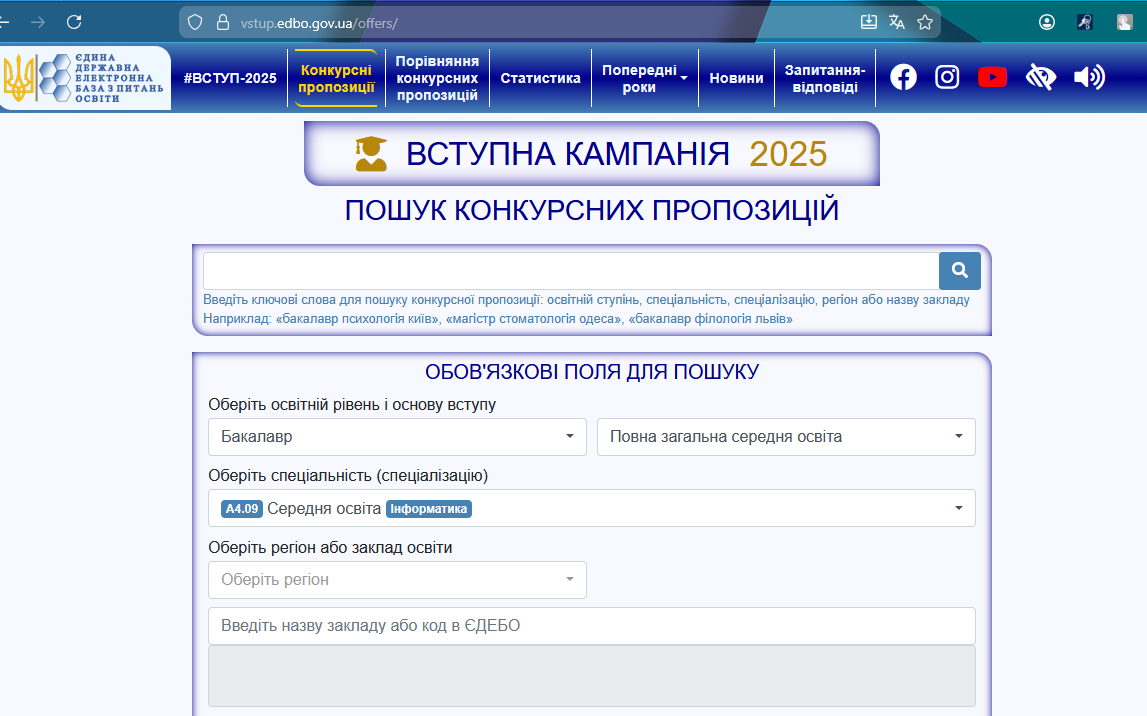
\includegraphics[width=\textwidth]{images/media/image8.png}
\caption{Інтерфейс пошуку конкурсних пропозицій у Єдиній державній електронній базі з питань освіти (ЄДЕБО)}
\label{fig:1.8}
\end{figure}

За результатами опрацювання інформації ЄДЕБО встановлено, що підготовка майбутніх учителів інформатики здійснюється у 38~закладах вищої освіти України (106~конкурсних пропозицій), серед яких переважають педагогічні університети (18~закладів), поряд із класичними університетами (14~закладів) та спеціалізованими ЗВО (6~закладів). Слід зауважити, що на офіційних вебсторінках окремих ЗВО (Класичний приватний університет, Мелітопольський державний педагогічний університет імені Богдана Хмельницького, Національний університет <<Чернігівський колегіум>> імені Т.~Г.~Шевченка, Сумський державний педагогічний університет імені А.~С.~Макаренка) відсутнє оприлюднення ОПП за відповідною спеціальністю, що ускладнило повноцінний порівняльний аналіз.

Порівняльний аналіз решти ОПП здійснювався за такими критеріями: (1)~наявність ІОР у формулюваннях результатів навчання та компетентностей; (2)~наявність окремих дисциплін або модулів, присвячених імерсивним технологіям; (3)~зміст дотичних дисциплін (комп'ютерна графіка, мультимедіа, STEM-освіта); (4)~форми використання цифрових ресурсів у навчальному процесі та практиках.

Аналіз засвідчив стійку тенденцію: практично в усіх ОПП цифрові технології декларуються як важливий компонент підготовки, однак імерсивні освітні ресурси не виокремлюються як самостійний об'єкт опанування чи специфічний результат професійної підготовки. У педагогічних університетах (Бердянський ДПУ, Житомирський ДУ, Херсонський ДУ) використання цифрових технологій і комп'ютерного моделювання декларується на рівні загальних результатів навчання, формулювання яких орієнтовані на здатність <<використовувати сучасні ІКТ>> або <<застосовувати цифрові освітні ресурси>> без конкретизації імерсивної складової. У програмах з підвищеним STEM-потенціалом (Волинський НУ, Черкаський НУ, КДПУ, КрНУ) зафіксовано дисципліни з комп'ютерної графіки, 3D-моделювання, STEM/STEAM-освіти, робототехніки, що створює сприятливі технологічні передумови, однак імерсивність залишається імпліцитною характеристикою. У спеціалізованих ЗВО (Кременчуцький НУ, Український ДУ імені Михайла Драгоманова) наявні курси <<Комп'ютерна графіка та доповнена реальність>>, <<Інноваційні технології навчання інформатики>>, у межах яких можливе використання елементів AR/VR, проте навіть тут імерсивні засоби розглядаються як окремі технологічні інструменти, а не як об'єкт цілеспрямованого педагогічного проєктування.

Форми використання цифрових та потенційно імерсивних ресурсів у проаналізованих ОПП зводяться переважно до трьох рівнів: інструментально-демонстраційного (лабораторні та практичні заняття з візуалізації об'єктів), проєктного (курсові роботи, STEM-проєкти з розробки цифрових моделей) та допоміжного під час педагогічних практик (мультимедійні презентації, інтерактивні вправи). В жодному з цих випадків ІОР не набувають статусу самостійного дидактичного інструмента з чітко визначеними дидактичними цілями, методами та критеріями оцінювання.

Узагальнені результати порівняльного аналізу ОПП подано в табл.~\ref{tab:opp_comparison}.

\begin{table}[!h]
\caption{Порівняльна характеристика інтеграції ІОР в ОПП підготовки майбутніх учителів інформатики}
\label{tab:opp_comparison}
\centering\small
\begin{tabularx}{\linewidth}{|p{3.2cm}|X|X|X|}
\hline
\hfil \textbf{Параметр} & \textbf{\makecell{Педагогічні\\ університети (18)}} & \textbf{\makecell{Класичні \\університети (14)}} & \textbf{\makecell{Спеціалізовані \\ЗВО (6)}} \\
\hline
ІОР у формулюваннях ОПП & Імпліцитно (<<ІКТ>>, <<цифрові ресурси>>) & Імпліцитно & Фрагментарно \\
\hline
Профільні ІОР-курси & Відсутні & Відсутні & Частково (1--2 ЗВО) \\
\hline
Дотичні дисципліни & Комп'ютерна графіка, мультимедіа & Комп'ютерне моделювання, STEM & AR/VR, цифровий дизайн \\
\hline
Форми використання ІОР & Демонстраційна, лабораторна & Проєктна, STEM & Проєктна, інноваційна \\
\hline
Рівень зрілості (рис.~\ref{fig:1.9}) & 1 (Імпліцитний) & 1--2 (Імпліцитний -- Інструментальний) & 2 (Інструментальний) \\
\hline
\end{tabularx}
\end{table}

Для систематизації отриманих результатів запропоновано модель рівнів зрілості інтеграції ІОР в освітньо-професійні програми підготовки вчителів інформатики (рис.~\ref{fig:1.9}). Модель вирізняє п'ять рівнів~--- від повної відсутності імерсивних компонентів (рівень~0) до наявності цілісної методики їх розробки з навчально-методичним забезпеченням (рівень~4). Як засвідчує проведений аналіз, абсолютна більшість вітчизняних ЗВО перебуває на рівнях 1--2, тоді як рівні 3--4 (проєктне створення ІОР та системна методика їх розробки) представлені одиничними випадками.

\begin{figure}[!h]
\centering
\resizebox{\textwidth}{!}{%
\begin{tikzpicture}[every node/.style={font=\small}]

% Vertical stack: Level 0 (bottom) to Level 4 (top)
\node[dia/lrbox=10cm, minimum height=1cm] (l0) at (0,0)
  {\textbf{Рівень 0: Відсутність} --- жодних цифрових/імерсивних компонентів};

\node[dia/lrbox=10cm, minimum height=1cm, above=0.8cm of l0] (l1)
  {\textbf{Рівень 1: Імпліцитний} --- загальні формулювання <<ІКТ-компетентність>> в ОПП, без конкретизації ІОР};

\node[dia/lrbox=10cm, minimum height=1cm, above=0.8cm of l1] (l2)
  {\textbf{Рівень 2: Інструментальний} --- окремі курси з елементами 3D/AR/VR (комп'ютерна графіка, мультимедіа)};

\node[dia/lrbox=10cm, minimum height=1cm, above=0.8cm of l2] (l3)
  {\textbf{Рівень 3: Проєктний} --- проєктне створення ІОР у вибіркових курсах};

\node[dia/lrbox=10cm, minimum height=1cm, above=0.8cm of l3] (l4)
  {\textbf{Рівень 4: Методичний} --- системна методика розробки ІОР із навчальним посібником та курсом};

% Arrows between levels
\draw[dia/arrow] (l0.north) -- (l1.south);
\draw[dia/arrow] (l1.north) -- (l2.south);
\draw[dia/arrow] (l2.north) -- (l3.south);
\draw[dia/arrow] (l3.north) -- (l4.south);

% Right-side labels: Ukrainian HEI distribution
\node[dia/label, right=0.5cm of l0.east, text width=5cm, align=left] {${\sim}$10\,\% ЗВО};
\node[dia/label, right=0.5cm of l1.east, text width=5cm, align=left] {${\sim}$60\,\% ЗВО (більшість)};
\node[dia/label, right=0.5cm of l2.east, text width=5cm, align=left] {${\sim}$25\,\% ЗВО (ВНУ, ЧНУ, КДПУ, КрНУ)};
\node[dia/label, right=0.5cm of l3.east, text width=5cm, align=left] {${\sim}$5\,\% ЗВО (КДПУ)};
\node[dia/label, right=0.5cm of l4.east, text width=5cm, align=left] {Цільовий рівень (внесок дисертації)};

% Left-side dashed bracket showing gap between levels 2 and 4
\draw[thick, dashed, red!70!black]
  ([xshift=-0.6cm]l3.south west) -- ([xshift=-0.6cm]l4.north west)
  node[midway, left=0.2cm, text width=2.5cm, align=right, font=\small\itshape, text=red!70!black]
  {розрив між практикою та методикою};

\end{tikzpicture}%
}

\caption{Модель рівнів зрілості інтеграції імерсивних освітніх ресурсів в ОПП підготовки вчителів інформатики}
\label{fig:1.9}
\end{figure}

\textbf{Дослідницька траєкторія КДПУ (2020--2024).} Найбільш послідовний і задокументований вітчизняний досвід інтеграції імерсивних освітніх ресурсів у підготовку вчителів інформатики сформовано в Криворізькому державному педагогічному університеті (КДПУ), де протягом 2020--2024~рр. здійснювалося систематичне дослідження цієї проблематики (рис.~\ref{fig:1.10}).

У~2020~р. було проведено порівняльний аналіз інструментів розробки WebAR (A-Frame, AR.js, Three.js, JSARToolKit, Babylon.js), що дозволило визначити технологічну основу для подальших педагогічних рішень~\cite{Shepiliev2020WebAR}. Наступного року розроблено та апробовано WebAR-квести профорієнтаційного спрямування з використанням маркерного та GPS-орієнтованого AR~\cite{Shepiliev2021Career}; паралельно сформульовано методи дизайну імерсивних електронних навчальних ресурсів~\cite{Semerikov2021IERDesignACM}. У~2022~р. опубліковано комплексну методологію проєктування ІОР, що включає 6-компонентну модель (аналіз~$\to$ вимоги~$\to$ вибір ПЗ~$\to$ розробка~$\to$ впровадження~$\to$ оцінювання) та 13-типову класифікацію імерсивних ресурсів~\cite{Semerikov2022IERDesign}. У~2024~р. розроблено триетапну методику навчання створення WebAR з інтегрованими моделями машинного навчання (TensorFlow.js, Teachable Machine, MindAR), що знаменує перехід від використання готових імерсивних інструментів до створення інтелектуальних освітніх застосунків~\cite{Semerikov2024WebARML_CoSinE, Semerikov2024WebAR_EduDim}.

\begin{figure}[!h]
\centering
\resizebox{\textwidth}{!}{%
\begin{tikzpicture}[every node/.style={font=\small}]

% Timeline axis
\draw[thick, -{Stealth[length=3mm]}] (-0.5,0) -- (16,0);

% Year markers
\foreach \x/\yr in {0.5/2020, 5/2021, 9.5/2022, 14/2024} {
  \draw[thick] (\x,0.15) -- (\x,-0.15);
  \node[below=0.3cm, font=\bfseries] at (\x,0) {\yr};
}

% Node boxes above timeline
\node[dia/lrbox=3.5cm, above=1cm of {(0.5,0)}] (n1) {%
  \textbf{Огляд інструментів WebAR}\\[2pt]
  A-Frame, AR.js, Three.js, JSARToolKit, Babylon.js\\[2pt]
%  {\footnotesize CEUR-WS Vol.~2832}%
};

\node[dia/lrbox=3.5cm, above=1cm of {(5,0)}] (n2) {%
  \textbf{Квести WebAR + методи дизайну ІОР}\\[2pt]
  маркерне та GPS-орієнтоване AR; методи проєктування\\[2pt]
%  {\footnotesize IOP JPhysConf; ACM DHW}%
};

\node[dia/lrbox=3.5cm, above=1cm of {(9.5,0)}] (n3) {%
  \textbf{6-компонентна модель проєктування ІОР}\\[2pt]
  аналіз~$\to$ вимоги~$\to$ ПЗ~$\to$ розробка~$\to$ впровадження~$\to$ оцінювання\\[2pt]
%  {\footnotesize Educational Dimension}%
};

\node[dia/lrbox=3.5cm, above=1cm of {(14,0)}] (n4) {%
  \textbf{Методика WebAR + ML}\\[2pt]
  TensorFlow.js, Teachable Machine, MindAR\\[2pt]
%  {\footnotesize CEUR-WS CoSinE; Educational Dimension}%
};

% Vertical connectors from timeline to boxes
\draw[dia/line] (0.5,0.15) -- (n1.south);
\draw[dia/line] (5,0.15) -- (n2.south);
\draw[dia/line] (9.5,0.15) -- (n3.south);
\draw[dia/line] (14,0.15) -- (n4.south);

% Horizontal progression arrows between boxes
\draw[dia/arrow] (n1.east) -- (n2.west);
\draw[dia/arrow] (n2.east) -- (n3.west);
\draw[dia/arrow] (n3.east) -- (n4.west);

% Bottom label: maturity progression
\node[below=1cm, font=\footnotesize\itshape] at (0.5,0) {Рівень 2};
\node[below=1cm, font=\footnotesize\itshape] at (5,0) {Рівень 2--3};
\node[below=1cm, font=\footnotesize\itshape] at (9.5,0) {Рівень 3};
\node[below=1cm, font=\footnotesize\itshape] at (14,0) {Рівень 3--4};

\end{tikzpicture}%
}

\caption{Дослідницька траєкторія КДПУ у сфері навчання розробки імерсивних освітніх ресурсів (2020--2024)}
\label{fig:1.10}
\end{figure}

Дослідницька траєкторія КДПУ засвідчує системну еволюцію від технологічного огляду інструментів (рівень~2 моделі зрілості) через проєктне створення ІОР (рівень~3) до формування цілісної методики їх розробки (рівень~3--4). Це єдиний задокументований вітчизняний приклад ЗВО, що послідовно просувається від фрагментарного використання імерсивних технологій до їх педагогічно обґрунтованої інтеграції у систему підготовки вчителів інформатики.

\textbf{Аналітичний синтез.} Результати порівняльного аналізу вітчизняних ОПП, розглянуті у контексті міжнародних тенденцій, дають підстави для таких узагальнень. По-перше, виявлений розрив між технологічним потенціалом освітніх програм і рівнем педагогічної реалізації ІОР не є суто українською проблемою~--- він відповідає глобальному патерну, зафіксованому у систематичних оглядах~\cite{Angelov2025Synergy, Taggart2023Makers}. По-друге, у термінах моделі TPACK~\cite{BeldaMedina2022TPACK}, аналіз ОПП виявляє системний дефіцит TPK-компоненту: програми формують окремо технологічні знання (TK~--- через курси комп'ютерної графіки, моделювання) і педагогічні знання (PK~--- через методику навчання інформатики), однак не забезпечують їх інтеграції у контексті імерсивних освітніх середовищ. По-третє, жодна з п'яти сутнісних характеристик ІОР, визначених у підрозділі~\ref{subsec:1.2} (інтерактивність, імерсивність, контекстуальність, візуалізація, адаптивність), не адресується як окремий об'єкт формування в проаналізованих ОПП.

Абсолютна більшість вітчизняних ЗВО перебуває на рівнях 0--2 моделі зрілості (рис.~\ref{fig:1.9}), тоді як цільовий рівень~4 (системна методика розробки ІОР із навчально-методичним забезпеченням) до цього часу не представлений у жодній ОПП. Досвід КДПУ~\cite{Shepiliev2020WebAR, Shepiliev2021Career, Semerikov2022IERDesign, Semerikov2024WebARML_CoSinE} засвідчує принципову можливість системного просування за цією шкалою, однак потребує оформлення в цілісну методику навчання.

%Узагальнені результати порівняльного аналізу освітньо-професійних програм представлено також у зведеній таблиці, яка подається у Додатку~А як аналітичне узагальнення.

Виявлені суперечності між задекларованою значущістю цифрових та імерсивних технологій в освітніх програмах і відсутністю системного підходу до формування відповідних професійних умінь обґрунтовують необхідність розроблення спеціально організованої методики навчання, спрямованої на формування в майбутніх учителів інформатики здатності цілеспрямовано проєктувати, дидактично осмислювати та педагогічно використовувати імерсивні освітні ресурси в освітньому процесі. Організаційно-педагогічні засади такої методики обґрунтовано у наступному розділі.

